\subsection{Glyph: \glyph{Annotation}}
\label{sec:annotation}

In \SBGNPDLone there are cases where the language does not capture everything the author wishes to convey.
This may be additional experimental detail or descriptions of mechanisms that cannot be fully described by the \PDl.
In this case the language provides the \glyph{annotation} glyph. This contains text and is associated with a particular glyph in a map.
Importantly, it is purely ``decoration'' and does alter the meaning the map.

\begin{glyphDescription}

\glyphSboTerm
SBO:0000550 ! annotation

\add{
\glyphIncoming
None.
}

\add{
\glyphOutgoing
None.
}

\glyphContainer
An \glyph{annotation} is represented by a rectangular shape with a folded corner, as shown in \fig{techref:annotation}.
This shape is linked to the annotated element via a callout (see Figure \ref{fig:techref:ex-annotation}).
The callout should overlap with the object it is annotating.

\glyphLabel
An \glyph{annotation} is identified by a label that is \corr{an unbordered box containing}{} a string of characters \corr{.
The characters}{that} may be distributed on several lines to improve readability.
The centre of the label must be placed on the centre of the shape.

\glyphAux
\corr{An \glyph{annotation} does not carry any auxiliary items}{None}.

\end{glyphDescription}

\begin{figure}[htb]
  \centering
  
\includegraphics{images/annotation}
  \caption{The \PD glyph for \glyph{annotation}.}
  \label{fig:techref:annotation}
\end{figure}

\begin{figure}[htb]
  \centering
  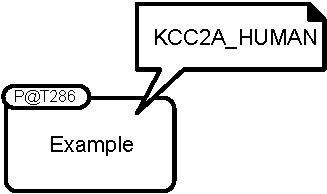
\includegraphics[scale = 0.8]{examples/ex-annotation}
  \caption{Example of \glyph{annotations} adding information to the
    description of the trans-phosphorylation of CaMKII. Note that
    three different types of links are used between annotation nodes
    and annotated elements. However, it is recommended to use a
    consistent scheme within a map.}
  \label{fig:techref:ex-annotation}
\end{figure}
